\section{Regressão Ordinal}

\subsection{Leituras Recomendadas}
\begin{frame}{Regressão Ordinal - Leituras Recomendadas}
	\begin{vfilleditems}
		\item \textcite{gelman2013bayesian} - Capítulo 16, Seção 16.2: Models for multivariate and multinomial responses
		\item \textcite{mcelreath2020statistical} - Capítulo 12, Seção 12.3: Ordered categorical outcomes
		\item \textcite{gelman2020regression} - Capítulo 15, Seção 15.5: Ordered and unordered categorical regression
		\item \textcite{Burkner_Vuorre_2019}
		\item \textcite{Semenova_2019}
	\end{vfilleditems}
\end{frame}

\subsection{O que é Regressão Ordinal?}
\begin{frame}{O que é Regressão Ordinal?}
	\textbf{Regressão ordinal} é um modelo de regressão para \textbf{dados discretos} e,
	mais especificamente, quando os \textbf{valores das variáveis dependentes têm uma "ordem natural"}.
	\vfill
	Por exemplo, pesquisas de opinião com seus intervalo de valores plausíveis de discordo-concordo ubíquos,
	ou uma percepção de dor do paciente.
\end{frame}
\begin{frame}{Por que não usar apenas Regressão Linear?}
	A principal razão para não usar regressão linear simples com resultados ordinais (variável dependente) é
	que as categorias de resposta de uma variável ordinal podem não ser \textbf{equidistantes}.
	Este é um pressuposto na regressão linear (e em quase todos os modelos que usam variáveis dependentes de métricas):
	a distância entre, por exemplo, 2 e 3 não é a mesma distância entre 1 e 2.
	\vfill
	Este pressuposto pode ser \textbf{violado em uma regressão ordinal}.
\end{frame}

\subsection{Como lidar com uma Variável Dependente Ordinal?}
\begin{frame}{Como lidar com uma Variável Dependente Ordinal?}
	Surpresa! Plot twist!
	\vfill
	Temos que fazer uma \textbf{transformação não-linear}.
\end{frame}

\begin{frame}{Função de Distribuição Cumulativa - FDC}
	No caso da regressão ordinal, primeiros temos que transformar a \textbf{variável
		dependente para uma escala cumulativa}.
	\vfill
	Para isso usamos a Função de Distribuição Cumulativa (FDC):

	$$P(Y \leq y) = \sum^y_{i=y_{\text{min}}} P(Y = i)$$

	A FDC é uma função \textbf{incremental monotônica} que representa a\textbf{ probabilidade
		de uma variável aleatória $Y$ tomar valores menores que um certo valor $y$}.
\end{frame}

\begin{frame}{\textit{Log-cumulative-odds}}
	Ainda sim, não é o suficiente.
	Precisamos aplicar a \textbf{função logit na FDC}:

	$$\mathrm{logit}(x) = \mathrm{logistic}^{-1}(x) = \ln\left(\frac{x}{1 -x}\right)$$

	onde $\ln$ é a função do log natural.
	\vfill
	A logit é o inverso da transformação logística: ela pega qualquer valor
	entre 0 e 1 (e.g. uma probabilidade) e transforma em um número real que
	chamamos de \textit{log-odds}\footnote{já vimos isso em regressão logística.}
	(log da chance).
	\vfill
	Como a transformação atua no FDC, chamados de \textbf{\textit{log-odds}} do FDC
	ou \textbf{\textit{log-cumulative-odds}} (log da chance cumulativa).
\end{frame}

\begin{frame}{$K-1$ Constantes}
	O que fazemos com essa tal de \textbf{\textit{log-cumulative-odds}}?
	\vfill
	Nos permite construir \textbf{diferentes constantes para os possíveis valores
		da nossa variável ordinal dependente}.
	Criamos uma \textbf{constante única para cada resultado $k \in K$}.
	\vfill
	Na verdade é $k \in K-1$. Note que o valor máximo de $Y$ sempre será $1$.
	O que se traduz em uma \textit{log-cumulative-odds} com valor $\infty$,
	pois $p=1$:

	$$\ln \frac{p}{1-p} = \ln \frac{1}{1-1} = \ln 0 = \infty$$

	Portanto, precisamos apenas de \textbf{$K-1$ constantes para $K$ possíveis valores
		que $Y$ pode tomar}.
\end{frame}

\begin{frame}{Violação da Equidistância}
	Como cada constante implica em um valor diferente de FDC para cada $k \in K$,
	podemos \textbf{violar o pressuposto da equidistância} que é ausente em quase
	todas as variáveis ordinais.
\end{frame}

\begin{frame}{Cut Points}
	Cada constante implica em uma \textit{log-cumulative-odds} para cada $k \in K$.
	Precisamos também \textbf{desfazer a natureza cumulativa das $K-1$ constantes}.
	Fazemos isso primeiramente \textbf{convertendo uma \textit{log-cumulative-odds}
		de volta para uma probabilidade válida com a função logística}:

	$$\mathrm{logit}^{-1}(x) = \mathrm{logistic}(x) = \frac{1}{1 + e^{-x}}$$

	Então finalmente removemos a natureza cumulativa da FDC ao
	\textbf{subtrairmos cada um dos $k$ \textit{cut points} (pontos de corte)
		do seu \textit{cut point} prévio $k-1$}:

	$$P(Y=k) = P(Y \leq k) - P(Y \leq k-1)$$
\end{frame}

\begin{frame}{Exemplo - Histograma\footnote{também chamado de \textbf{f}unção de \textbf{d}istribuição de \textbf{p}robabilidade (FDP).} de uma Variável Ordinal}
	\centering
	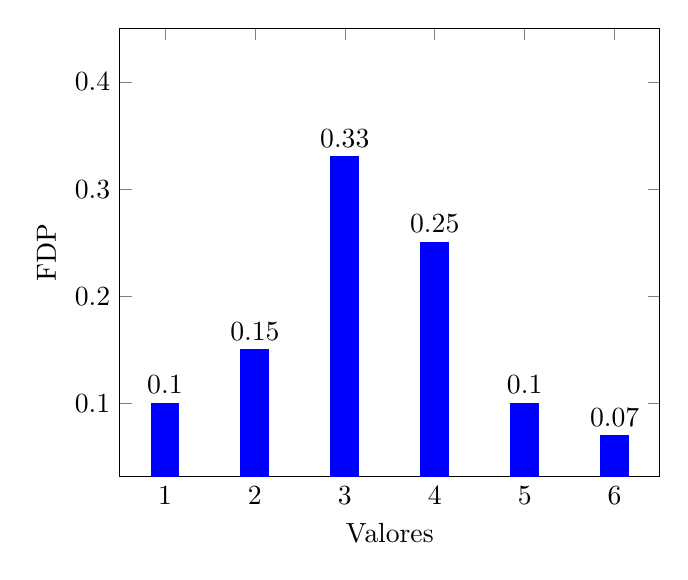
\begin{tikzpicture}[ybar]
		\begin{axis}[
				nodes near coords={\pgfmathprintnumber[fixed,precision=3]{\pgfplotspointmeta}},
				xlabel=Valores,
				ylabel=FDP,
				xtick={1,2,3,4,5,6},
				ytick={0.1,0.2,0.3,0.4},
				ymax=0.45]
			\addplot [draw=blue, fill=blue] coordinates {
					(1, 0.10)
					(2, 0.15)
					(3, 0.33)
					(4, 0.25)
					(5, 0.10)
					(6, 0.07)
				};
		\end{axis}
	\end{tikzpicture}
\end{frame}

\begin{frame}{Exemplo - FDC versus \textit{Log-cumulative-odds}}
	\begin{columns}
		\begin{column}{0.5\textwidth}
			\centering
			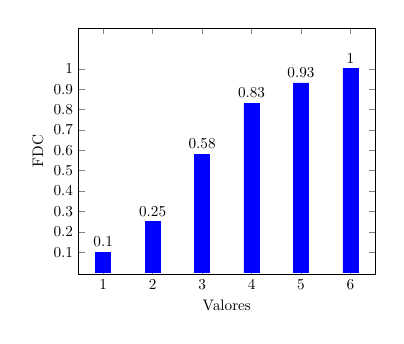
\begin{tikzpicture}[
					ybar,
					scale=0.55]
				\begin{axis}[
						nodes near coords={\pgfmathprintnumber[fixed,precision=3]{\pgfplotspointmeta}},
						xlabel=Valores,
						ylabel=FDC,
						xtick={1,2,3,4,5,6},
						ytick={0.1,0.2,0.3,0.4,0.5,0.6,0.7,0.8,0.9,1.0},
						ymax=1.2]
					\addplot [draw=blue, fill=blue] coordinates {
							(1, 0.10)
							(2, 0.25)
							(3, 0.58)
							(4, 0.83)
							(5, 0.93)
							(6, 1.00)
						};
				\end{axis}
			\end{tikzpicture}
		\end{column}
		\begin{column}{0.5\textwidth}
			\centering
			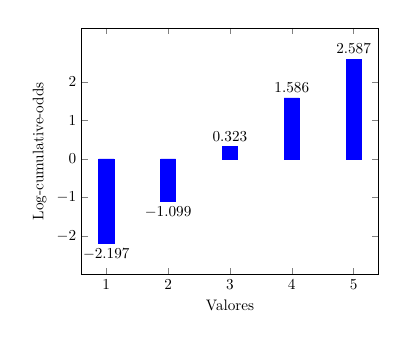
\begin{tikzpicture}[
					ybar,
					scale=0.55]
				\begin{axis}[
						nodes near coords={\pgfmathprintnumber[fixed,precision=3]{\pgfplotspointmeta}},
						xlabel=Valores,
						ylabel=Log-cumulative-odds,
						xtick={1,2,3,4,5,6},
						ytick={-2,-1,0,1,2},
						ymax=3.4,
						ymin=-3]
					\addplot [draw=blue, fill=blue] coordinates {
							(1, -2.19722)
							(2, -1.09861)
							(3, 0.322773)
							(4, 1.58563)
							(5, 2.58669)
							(6, 10.0)
						};
				\end{axis}
			\end{tikzpicture}
		\end{column}
	\end{columns}
\end{frame}

\subsection{Adicionando Coeficientes $\beta$}
\begin{frame}{Adicionando Coeficientes $\beta$}
	Com o pressuposto da equidistância resolvido com as $K-1$ constantes
	podemos adicionar coeficientes como efeitos de variáveis independentes
	na nossa regressão ordinal.
\end{frame}

\begin{frame}{Mais \textit{Log-cumulative-odds}}
	Transformamos todas as constantes em \textit{log-cumulative-odds} para
	que possamos adicionar efeitos (coeficientes multiplicando uma variável
	independente) à taxas basais (constantes).
	\vfill
	Para cada $k \in K-1$, nos calculamos:

	$$\phi_k = \alpha_k + \beta_i x_i$$

	onde $\alpha_k$ é a \textit{log-cumulative-odds} para as $k \in K-1$ constantes,
	$\beta_i$ é o coeficiente para a $i$nésima variável independente $x$.
	\vfill
	Por fim, $\phi_k$ representa o preditor linear para a $k$nésima constante.
\end{frame}

\begin{frame}{Notação de Matriz}
	Tudo isso fica muito mais elegante e computacionalmente eficiente se
	colocarmos em notação de matriz e vetor:

	$$\boldsymbol{\phi} = \boldsymbol{\alpha} + \mathbf{X} \cdot \boldsymbol{\beta}$$

	onde $\boldsymbol{\phi}$, $\boldsymbol{\alpha}$ e $\boldsymbol{\beta}$\footnote{note que tanto os coeficientes quanto as constantes terão que ser interpretados em chances igual a regressão logística.}
	são vetores e $\mathbf{X}$ é a matriz de dados em que cada linha é uma
	observação e cada coluna uma variável independente.
\end{frame}

\subsection{Modelo Completo}
\begin{frame}{Modelo Completo}
	\footnotesize
	$$
		\begin{aligned}
			\mathbf{y}          & \sim \text{Categórica}(\mathbf{p})                                        \\
			\mathbf{p}          & = \mathrm{logistica}(\boldsymbol{\phi})                                   \\
			\boldsymbol{\phi}   & = \boldsymbol{\alpha} + \mathbf{X} \cdot \boldsymbol{\beta}               \\
			\alpha_1            & = \mathrm{FDC}(y_1)                                                       \\
			\alpha_k            & = \mathrm{FDC}(y_k) - \mathrm{FDC}(y_{k-1}) \mathrm{ para } 1 < k < K-1   \\
			\alpha_{K-1}        & = 1 - \mathrm{FDC}(y_{K-1})                                               \\
			\boldsymbol{\alpha} & \sim \text{Normal}(\mu_\alpha, \sigma_\alpha)                             \\
			\boldsymbol{\beta}  & \sim \text{Normal}(\mu_{\boldsymbol{\beta}}, \sigma_{\boldsymbol{\beta}})
		\end{aligned}
	$$
	\begin{vfilleditems}
		\item \footnotesize  $\mathbf{y}$: variável dependente ordinal discreta
		\item \footnotesize  $\mathbf{p}$: vetor de probabilidade de tamanho $K$
		\item \footnotesize  $K$: número de valores possíveis que $\mathbf{y}$ pode tomar, i.e. número de valores ordenados discretos
		\item \footnotesize  $\boldsymbol{\phi}$: \textit{log-cumulative-odds}, i.e. os \textit{cut points} considerando as constantes e os efeitos das variáveis independentes
		\item \footnotesize  $\alpha_k$: constante em \textit{log-cumulative-odds} para cada $k \in K-1$
		\item \footnotesize  $\mathbf{X}$: matriz de dados das variáveis independentes
		\item \footnotesize  $\boldsymbol{\beta}$: vetor de coeficientes do mesmo tamanho do número de colunas em $\mathbf{X}$
	\end{vfilleditems}
\end{frame}

\subsection{Regressão Ordinal no \texttt{brms}}
\begin{frame}[fragile]{Regressão Ordinal no \href{https://paul-buerkner.github.io/brms/}{\texttt{brms}}}
	Usamos a função \texttt{brm()} com os argumentos \texttt{family = cumulative(link = "logit")}:
	\vfill
	\begin{lstlisting}[basicstyle=\small]
    modelo_ordinal <- brm(
    y ~ ...,
    data = df,
    family = @cumulative(link = "logit")@,
    prior = c(
        set_prior("...", class = "b", coef = "..."),
                ...
        set_prior("...", class = "b", coef = "intercept")
        )
    )
    \end{lstlisting}
\end{frame}
